\documentclass{beamer}
\usepackage{beamerthemesplit}
\usepackage{epstopdf}
\usepackage{natbib}
\usepackage{stackengine}
\bibpunct{(}{)}{;}{a}{,}{,~}
\usepackage{amsmath,array,booktabs,supertabular,dcolumn,pifont}
\usepackage{rotating,multirow}
\usepackage{transparent,soul}
\usepackage{wasysym} % for \permil
\usepackage{subfigure}
\usepackage{ragged2e}
\definecolor{Gray}{gray}{0.9}
\usepackage{colortbl}
\definecolor{lightgray}{gray}{0.9}
\usepackage{array}
\usepackage{makecell}
\usepackage{verbatim}
\newcolumntype{C}{>{\centering\arraybackslash}p{4em}}
\usepackage[multidot]{grffile}
\newcolumntype{d}{D{.}{.}{2.5}}
\newcolumntype{s}{D{.}{.}{1.2}}
\newcolumntype{i}{D{.}{.}{3.0}}


\definecolor{dkgreen}{rgb}{0,0.6,0}
\definecolor{gray}{rgb}{0.5,0.5,0.5}
\definecolor{mauve}{rgb}{0.58,0,0.82}


% Custom colors %%%%%%%%%%%%%%%%%%%%%%%%%%%%%%%%%%%%%%%%%%%%%%%%%%%%%%%%%%%%%%%
\definecolor{DarkRed}{rgb}{0.60,0.00,0.00}
\definecolor{DarkGreen}{rgb}{0.0,0.70,0.0}
\definecolor{DarkBlue}{rgb}{0.0,0.0,0.6}
\definecolor{Gold}{rgb}{0.57,0.49,0.23}

% ORNL 
\definecolor{ORNLCCSI-Green}{rgb}{0.16,0.46,0.29}
% University of Tennessee
\definecolor{UTK-Orange}{rgb}     {0.16,0.46,0.29}
\definecolor{UTK-White}{rgb}      {1.000,1.000,1.000} 
\definecolor{UTK-Smokey}{rgb}     {0.345,0.349,0.357} 
\definecolor{UTK-Valley}{rgb}     {0.000,0.455,0.435} 

\setbeamercolor{structure}{bg=UTK-White,fg=UTK-Orange}
\setbeamercolor{block title}{bg=UTK-Smokey,fg=UTK-Orange}
\setbeamercolor{block body}{bg=UTK-Smokey,fg=UTK-Valley}
\setbeamercolor{block body alerted}{bg=UTK-Orange,fg=UTK-Smokey}
\setbeamercolor{alerted text}{bg=UTK-Smokey,fg=UTK-Orange}
\setbeamercolor{frametitle}{fg=UTK-White}
\setbeamercolor{normal text}{fg=UTK-Smokey}
%


\mode<presentation>
{
 %
 % Themes without navigation bar:
 %\usetheme{default}
  \usetheme{boxes}
 %\usetheme{classic}
 %\usetheme{Bergen}
 %\usetheme{Madrid}
 %\usetheme{Pittsburgh}
 %\usetheme{Rochester}
 %
 % Themes with a tree-like navigation bar:
 %\usetheme{Antibes}
 %\usetheme{JuanLesPins}
 %\usetheme{Montpellier}
 %
 % Themes with a TOC sidebar
 %\usetheme{Berkeley}
 %\usetheme{PaloAlto}
 %\usetheme{Goettingen}
 %\usetheme{Marburg}
 %\usetheme{Hannover}
 %
 % Themes with mini frame navigation
 %\usetheme{Berlin}
 %\usetheme{Ilmenau}
 %\usetheme{Dresden}
 %\usetheme{Darmstadt}
 %\usetheme{Frankfurt}% Pretty good
 %\usetheme{Singapore}
 %\usetheme{Szeged}
 %
 % Themes with section and subsection titles:
 %\usetheme{Copenhagen}
 %\usetheme{Luebeck}
 %\usetheme{Malmoe}
 %\usetheme{Warsaw}
 %
 %\usecolortheme{lily}
 %
 %\usefonttheme{sans}
 %\usefonttheme{serif}
 %\usefonttheme{structurebold}
 %\beamersetaveragebackground{black}
 %\beamertemplatesolidbackgroundcolor{black}
 %\beamertemplateshadingbackground{blue}{white}
}

\setbeamertemplate{blocks}[rounded][shadow=true]
\setbeamersize{text margin left=0.3cm,text margin right=0.3cm}
% Remove navigation symbols
\beamertemplatenavigationsymbolsempty
% or
%\setbeamertemplate{navigation symbols}{}
%


\title[DNN for Wildfire Mapping]{Wildfire Mapping in Interior Alaska Using Deep Neural Networks on Imbalanced Datasets}
\author{
Zachary~L.~Langford$^{1}$,
Jitendra~Kumar$^{2,1}$,
and
Forrest~M.~Hoffman$^{2,3}$
}
\institute{
$^{1}$Bredesen~Center, University~of~Tennessee~Knoxville;
$^{2}$Climate~Change~Science~Institute, Oak~Ridge~National~Laboratory;
and
$^{3}$Dept.~of~Civil~\&~Environmental~Engineering, University~of~Tennessee~Knoxville
}
\date{November 18, 2018}

\begin{document}


\begin{frame}
 %\setbeamercolor{alerted text}{fg=white}
 \titlepage
 \vskip-0.20in

 % UTK - ORNL - CCSI
 \centerline{\hfill
  
\includegraphics[height=0.12\paperheight]{logos/UTK_horizontal_logo_FMH.png}
  \hfill
  
\includegraphics[height=0.11\paperheight]{logos/ORNL_logo.pdf}
  \hfill
  
\includegraphics[height=0.12\paperheight]{logos/CCSI_Text_Logo_transparent.png}
  \hfill
 }
\end{frame}

% Slides start here 
%%%%%%%%%%%%%%%%%%%%%%%%%%%%%%%%%
%\section{Introduction and Datasets}
\begin{frame}
  \frametitle{Research Questions}
  \begin{itemize}
  \footnotesize
   \item Can we map wildfires in Interior Alaska based on imbalanced classes (wildfire vs. no-wildfire)?
   \item Does a weight-selection strategy on a deep MLP model based on the imbalanced class improve performance? 
  \end{itemize}

\begin{columns}[T]
\begin{column}{.60\textwidth}
  \centering
             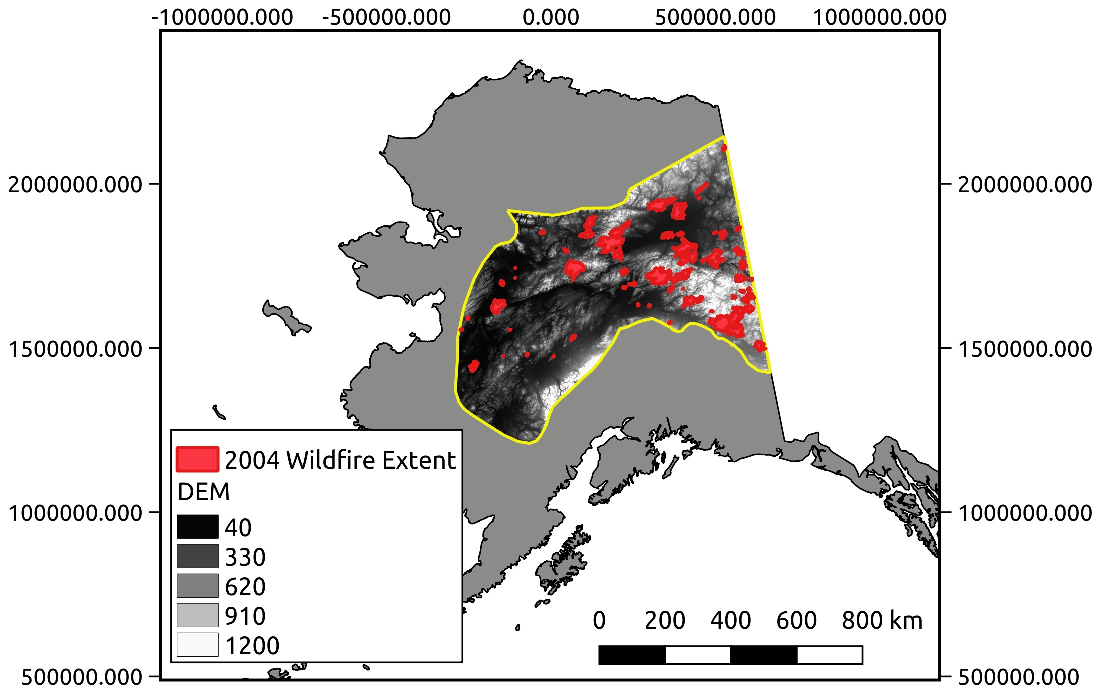
\includegraphics[width=\textwidth]{figs/study_area}
\end{column}%
\hfill%
\begin{column}{.40\textwidth}
Overview
\scriptsize
\begin{itemize}
 \item Bounded by Interior Alaska, based on climate conditions. 
 \item Background class (no-wildfire) significantly outweighs the wildfire class for 2004.
 \item 1,742,618 no-wildfire pixels and 105,072 wildfire pixels (500$\times$500~m).
 \item Select MLP weights during training that reflect the imbalanced class. 
 \item \textbf{Added segmentation algorithm and XGBoost for comparison.}
\end{itemize}
  
\end{column}%
\end{columns}
  
\end{frame}

%%%%%%%%%%%%%%%%%%%%%%%%%%%%%%%%%
\begin{frame}
  \frametitle{Motivation}
  \begin{itemize}
  \footnotesize
   \item Need to \textbf{provide unique datasets} for model parameterization on 
topics ranging from watershed hydrology to plant physiology that is being 
adopted by DOE's Earth System Modeling program and​ Next​ 
Generation​ Ecosystem​ Experiment​ (NGEE)​ Arctic 
(\url{https://ngee-arctic.ornl.gov/}).
  \end{itemize}

    \begin{columns}[T]
    \begin{column}{.5\textwidth}
     
   
   \centering
   \vspace{-0.2cm}
   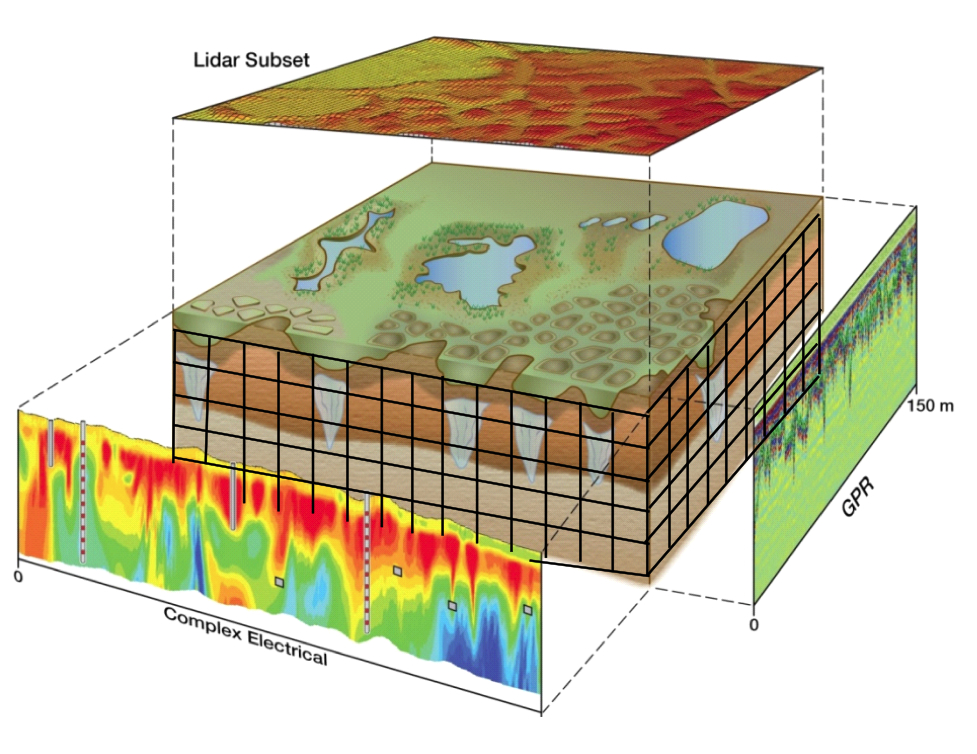
\includegraphics[width=1.0\textwidth]{figs/studyingperm.jpg}

    \end{column}
    \begin{column}{.5\textwidth}
    \vspace{-0.2cm}
    
 
    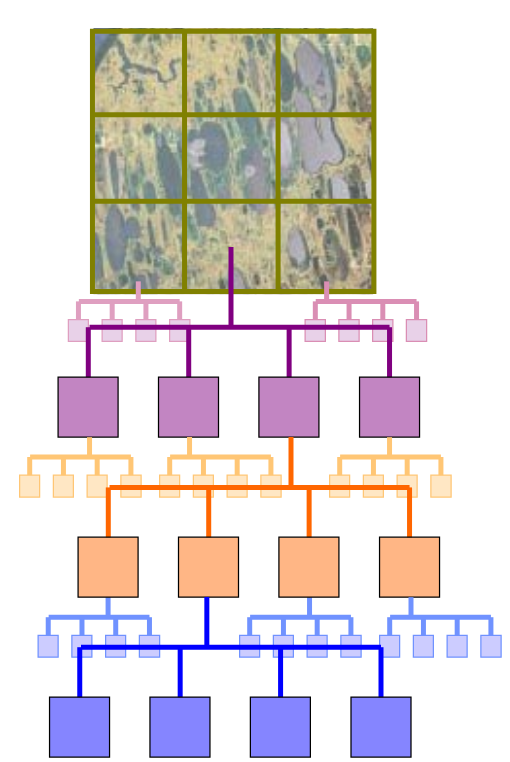
\includegraphics[width=0.7\textwidth]{figs/ngee_scaling.png}
    
   
    \end{column}
  \end{columns}

\footnotesize{NGEE Arctic Mission Statement 
\url{https://ngee-arctic.ornl.gov/mission}}
  
\end{frame}

%%%%%%%%%%%%%%%%%%%%%%%%%%%%%%%%%
\begin{frame}
  \frametitle{Class Imbalance Problem}


\begin{columns}[T]
    \begin{column}{.5\textwidth}
     
    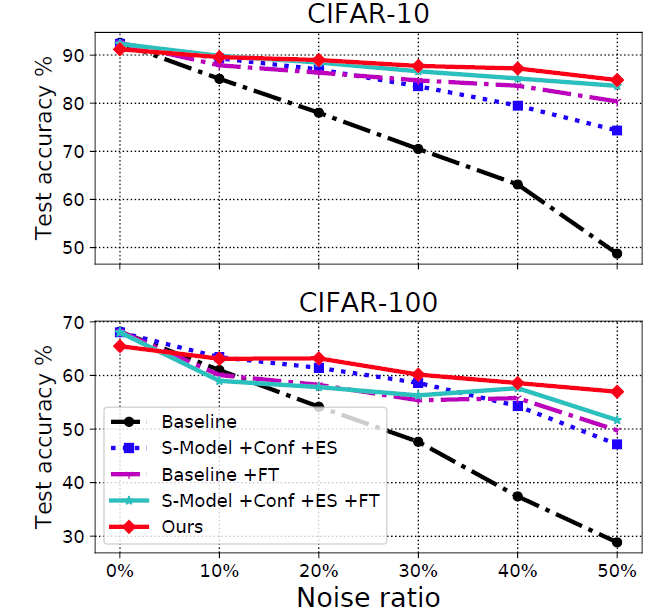
\includegraphics[width=1.0\textwidth]{figs/icml_2018.PNG}
  \\
  \tiny
  Learning to Reweight Examples for Robust Deep Learning 
\citep{pmlr-v80-ren18a}
    \end{column}
    \begin{column}{.5\textwidth}
    \scriptsize
\begin{itemize}
 \item Imbalanced data classification
exists where one class (e.g., burned areas) contains a much
smaller sample size than the others (e.g., unburned areas) in
classification. It poses a great challenge for DNN architectures,
due to the difficulty in recognizing the minority class \citep{Sze-To2017}.
\item However, there has been a significant amount of research
performed on the class imbalance problems using dataset
resampling \citep{Chawla02smote:synthetic}, cost-sensitive weighting 
\citep{Ting:2000:CSC:645529.657944}, and few-shot
learning \citep{Sachin2017}.
\item To
determine the weights, \cite{pmlr-v80-ren18a} method
performs a meta gradient descent step on the
current mini-batch example weights to minimize the loss on
a clean unbiased validation set.
\end{itemize}
    
    \end{column}
\end{columns}

\end{frame}

%%%%%%%%%%%%%%%%%%%%%%%%%%%%%%%%%
\begin{frame}
  \frametitle{Alaska Wildfires -- 2004}
  \begin{itemize}

\item One of the warmest and driest summers on record.
\item Most lightning strikes recorded during summer. 
\item Wildland fires burned the largest area in recorded Alaska history.
\item Total fires were 701 and area burned 6,600,000 acres.
\end{itemize}

\begin{columns}[T]
    \begin{column}{.5\textwidth}
     
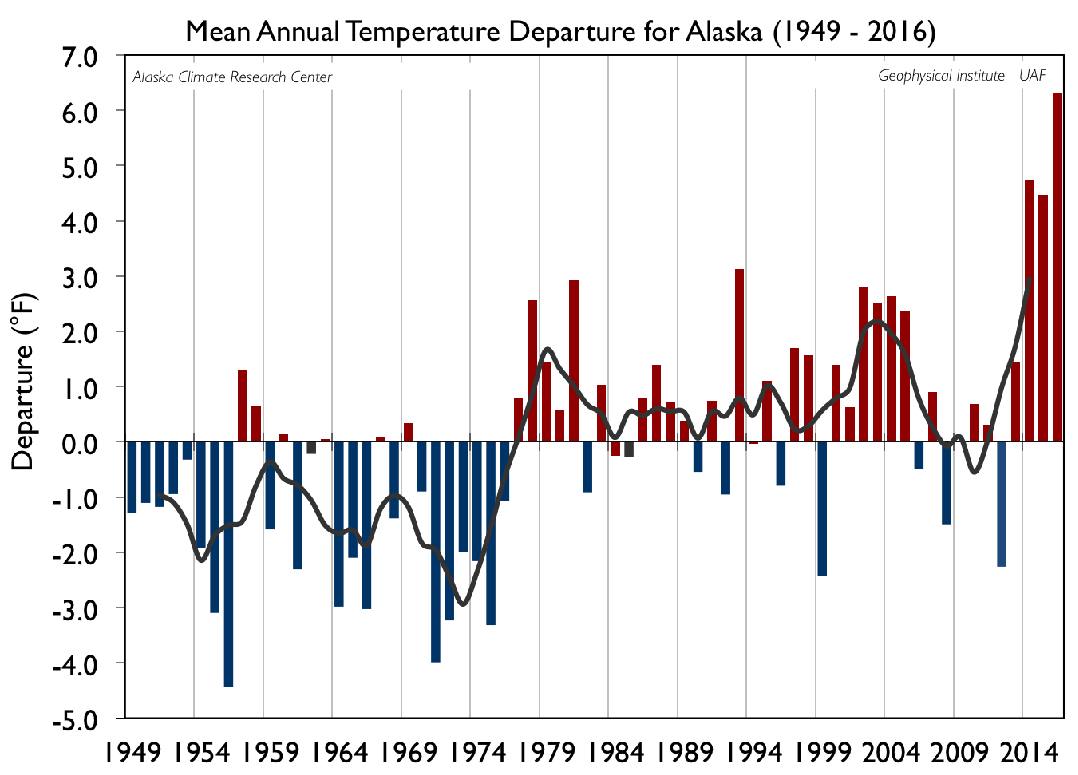
\includegraphics[width=1.0\textwidth]{figs/StateWide_Change_1949-2016_F.pdf}
  \\
  \tiny
  Departure from average temperature across Alaska for every year since 1949. 
(Image Source: Alaska Climate Research Center)
    \end{column}
    \begin{column}{.5\textwidth}
    
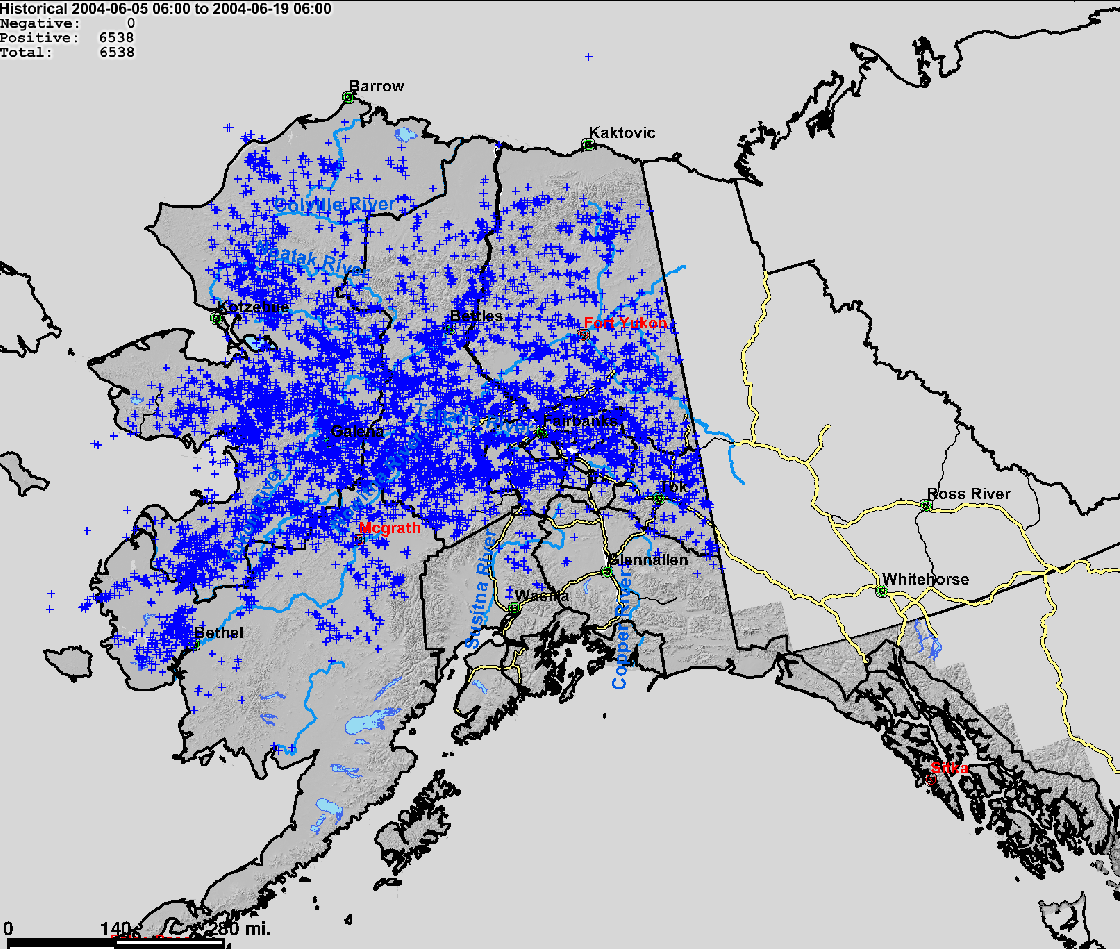
\includegraphics[width=1.00\textwidth]{figs/lighting_ak}
   \\
   \tiny 
    Number of lightnings strikes (6,538) in Alaska from June 5--19, 2004. 
    The grand total was over 147,642 strikes. 
    \end{column}
\end{columns}
\end{frame} 
%%%%%%%%%%%%%%%%%%%%%%%%%%%%%%%%%
\begin{frame}
  \frametitle{Geospatial Datasets}
  \vspace{-0.3cm}
\footnotesize
We used Google Earth Engine (GEE) for processing images. 
Two types of datasets were used:
\begin{itemize}
 \item MODIS: MOD09A1 (Surface Reflectance 8-Day L3 Global 500m)
  \item MODIS: MOD11A2 (Land Surface Temperature and Emissivity 8-Day L3 Global 1km)
\end{itemize}

\begin{columns}[T]
    \begin{column}{.4\textwidth}

  \tiny
        \begin{tabular}{p{10mm}p{10mm}p{15mm}} \toprule
        Description    & Resolution   & Variable \\ \midrule
        MOD09A1  

       & 500~m at 8 days & NDVI \\ \cmidrule(l){2-3}
       & 500~m at 8 days & EVI \\ \cmidrule(l){2-3}
       & 500~m at 8 days & SAVI \\ \cmidrule(l){2-3}

       & 500~m at 8 days & Bands 1--7 (459--2155 nm) \\ \cmidrule(l){1-3}
       MOD11A2
       & 1~km at 8 days & Daytime LST (Kelvin) \\ \cmidrule(l){1-3}
       MTBS
       & annual/500~m & Fire Boundary \\ \cmidrule(l){1-3}
       
       \bottomrule
    \end{tabular}
    \end{column}
    \begin{column}{.6\textwidth}

     \centering
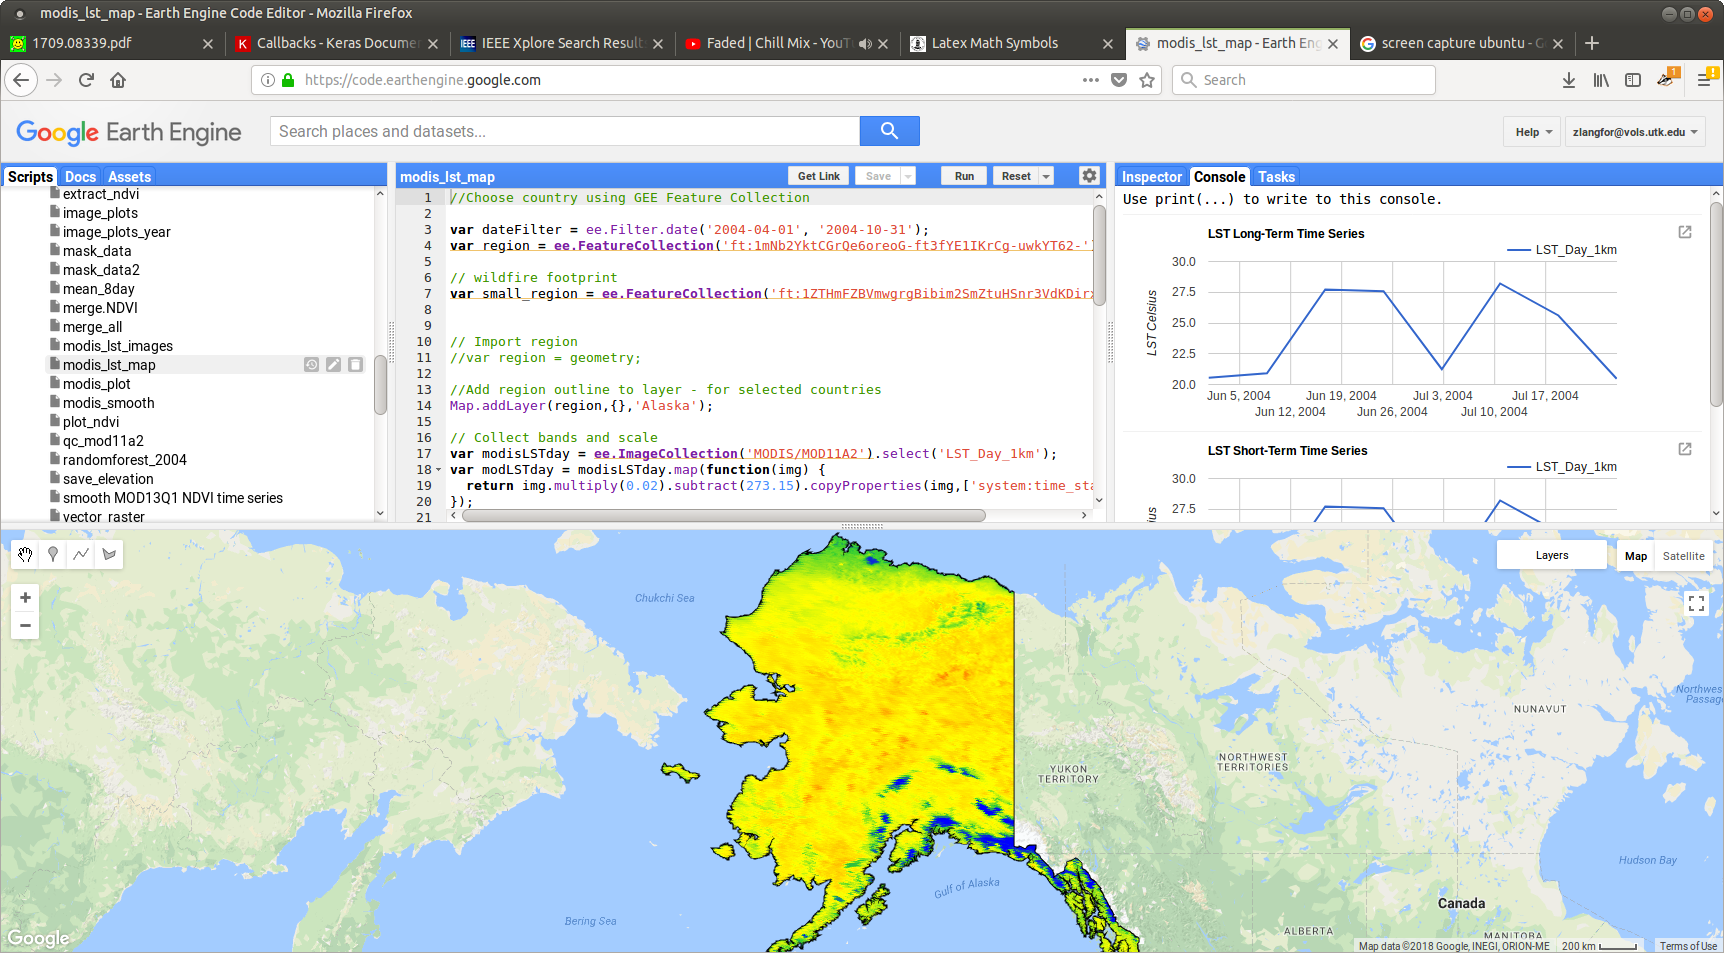
\includegraphics[width=1.0\textwidth]{figs/gee_ak.png}
\\

Google Earth Engine JavaScript API

    \end{column}
  \end{columns}
   
\end{frame}

%%%%%%%%%%%%%%%%%%%%%%%%%%%%%%%%%
\begin{frame}
  \frametitle{Image Processing}
\begin{columns}[T]
    \begin{column}{.5\textwidth}
    
  \centering
  \scriptsize 
\vspace{-0.2cm}
\begin{itemize}
 \item Increased resolution to 500~m for all datasets, GEE performs nearest neighbor resampling. 
 \item Linear interpolation for missing values.  
 \item Savitzky-Golay filter was applied to smooth out noise.
 \item Converted MTBS vector boundary to raster pixels. 
\end{itemize}
\vspace{-0.2cm}
   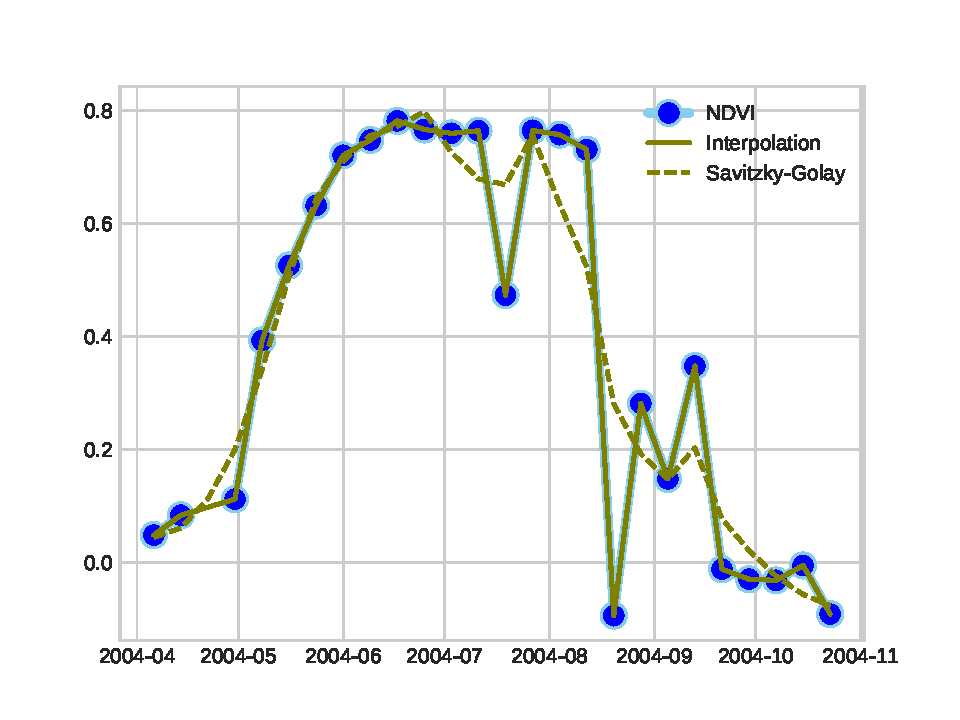
\includegraphics[width=1.0\textwidth]{figs/dallcity2004_fire}
\\ 
\tiny 
Example image processing workflow applied to a large wildfire, which occurred on July 6, 2004.
    \end{column}
    \begin{column}{.5\textwidth}
\vspace{-0.2cm}
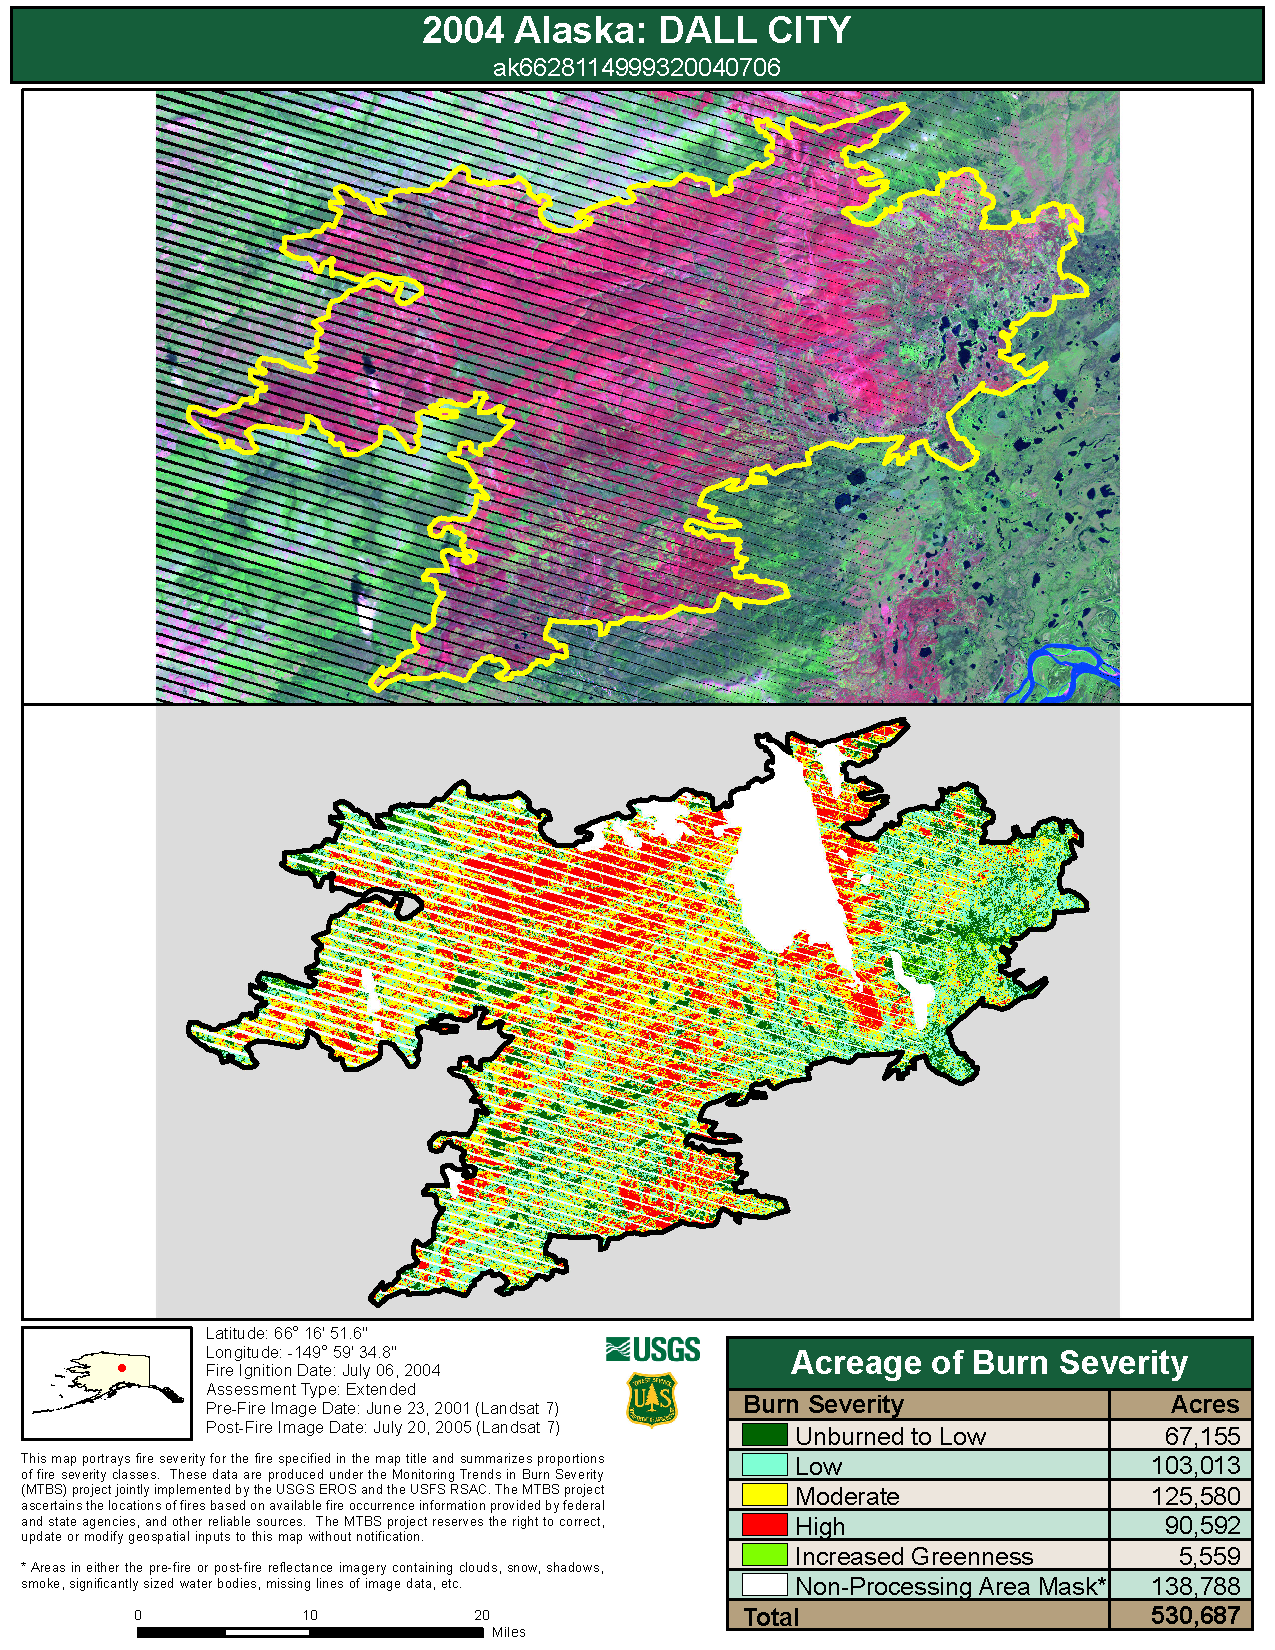
\includegraphics[width=1.0\textwidth]{figs/ak6628114999320040706_map}
\\ 
\tiny 
Fire severity for the Boundary fire based on Landsat 7. (Source: USGS and US Forest Service)

    \end{column}
  \end{columns}
\end{frame}

%%%%%%%%%%%%%%%%%%%%%%%%%%%%%%%%%
\begin{frame}
  \frametitle{Validation-Loss Strategy}
  \tiny
%Classification: $\bullet$ no wildfire (0) $\bullet$ wildfire (1) \\
%VL strategy splits the training data into separate distributions for \textbf{selecting} weights.

\centering
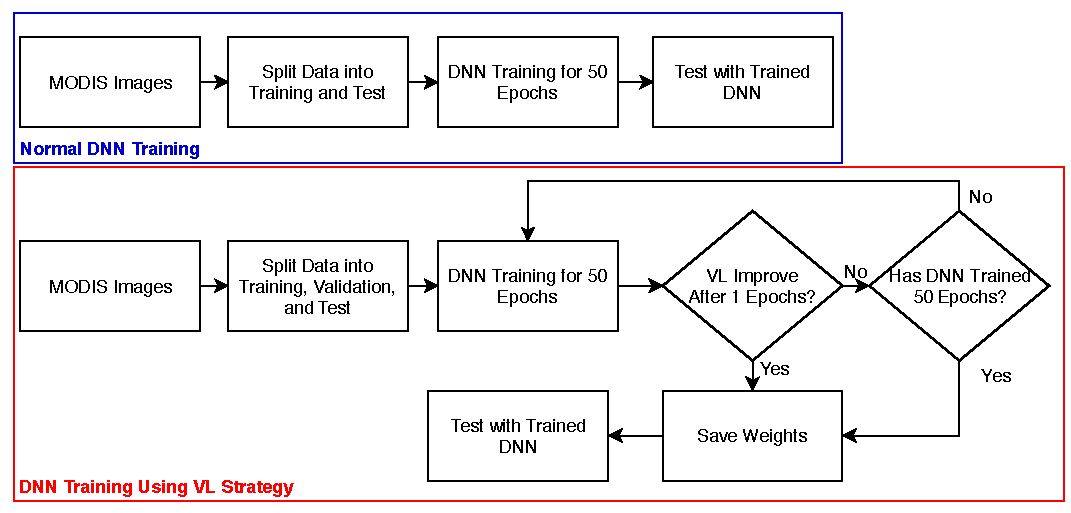
\includegraphics[width=0.9\textwidth]{figs/icdm_dnn}


 \hspace{-1cm}
 \scriptsize
 \begin{itemize}
  \item Weight selection strategy from \cite{Sze-To2017}.
\item Normal DNN training loss/accuracy measured on training data. 
\item VL strategy splits data into equal parts per class for for \textbf{selecting} weights.
\item Split data equally between classes for measuring VL.
\item Done by: keras.callbacks.ModelCheckpoint(filepath, monitor='val\_loss', 
verbose=0, save\_best\_only=False, save\_weights\_only=False, mode='auto', 
period=1)
 \end{itemize}



\end{frame}

%%%%%%%%%%%%%%%%%%%%%%%%%%%%%%%%%
\begin{frame}
  \frametitle{Deep MLP Models}
  
\scriptsize
self.model = Sequential() \\
self.model.add(Dense(60, activation=relu, kernel$\_$initializer=normal, 
input$\_$dim=nb$\_$bands)) \\
self.model.add(Dense(30, kernel$\_$initializer=normal, activation=relu)) \\
self.model.add(Dense(10, kernel$\_$initializer=normal, activation=relu)) \\
self.model.add(Dense(nb$\_$classes, kernel$\_$initializer=normal, activation=softmax)) \\
self.model.summary() \\
self.model.compile(optimizer=Adam(),
		loss=sparse$\_$categorical$\_$crossentropy,
		metrics=[accuracy])

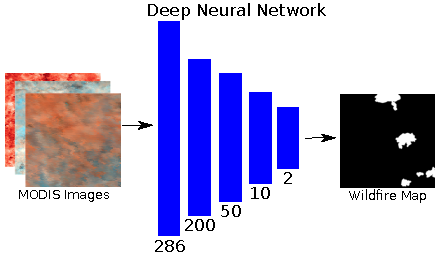
\includegraphics[width=0.8\textwidth]{figs/dnn_fig}



\end{frame} 



%%%%%%%%%%%%%%%%%%%%%%%%%%%%%%%%%
\begin{frame}
  \frametitle{Training/Testing/Validation Datasets}


\begin{columns}[T]
    \begin{column}{.6\textwidth}
 \vspace{-0.25cm}   
\small
    \begin{tabular}{ | l | l | l | l |}
    \hline

    Dataset & No-Fire & Fire & Percentage\\ \hline
%%%%%%%%%%%%%%%%%%%%%%%%%%%%
    Dataset-0 Train & 1154333 & 70493 & 75\% \\ 
    Dataset-0 Test  & 427115 & 26356 & 25\% \\ 

    Dataset-0 Validation & 7947 & 7947 & 10\% \\ \hline
%%%%%%%%%%%%%%%%%%%%%%%%%%%%
    Dataset-1 Train & 384375 & 23477 & 25\% \\ 

    Dataset-1 Test  & 1282862 & 78702 & 75\% \\ 

    Dataset-1 Validation & 2617 & 2617 & 10\% \\ \hline
%%%%%%%%%%%%%%%%%%%%%%%%%%%%
    Single Wildfire & 9724 & 276 & $<$1\% \\ 
    
    \hline
    \end{tabular}

  \centering
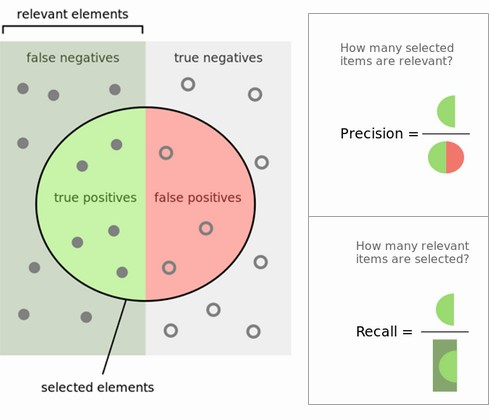
\includegraphics[width=0.8\textwidth]{figs/precision-recall-relevant-selected.jpg}
\\
\tiny{source:\url{https://en.wikipedia.org/wiki/Precision_and_recall}}

    \end{column}

    \begin{column}{.4\textwidth}
\vspace{3.0cm}

\begin{itemize}
\scriptsize
\item Number of pixels (500$\times$500) used for training, testing, and validation.
\item The validation column was only applied when using the VL strategy.
\item Precision --  high value means that an algorithm returned substantially more relevant results than irrelevant ones.
\item Recall -- high value means that an algorithm returned most of the relevant results
\end{itemize}


    \end{column}
  \end{columns}


\end{frame}

%%%%%%%%%%%%%%%%%%%%%%%%%%%%%%%%%

\begin{frame}
  \frametitle{Results -- MLP Training}

\begin{figure}
  
  \stackunder[5pt]{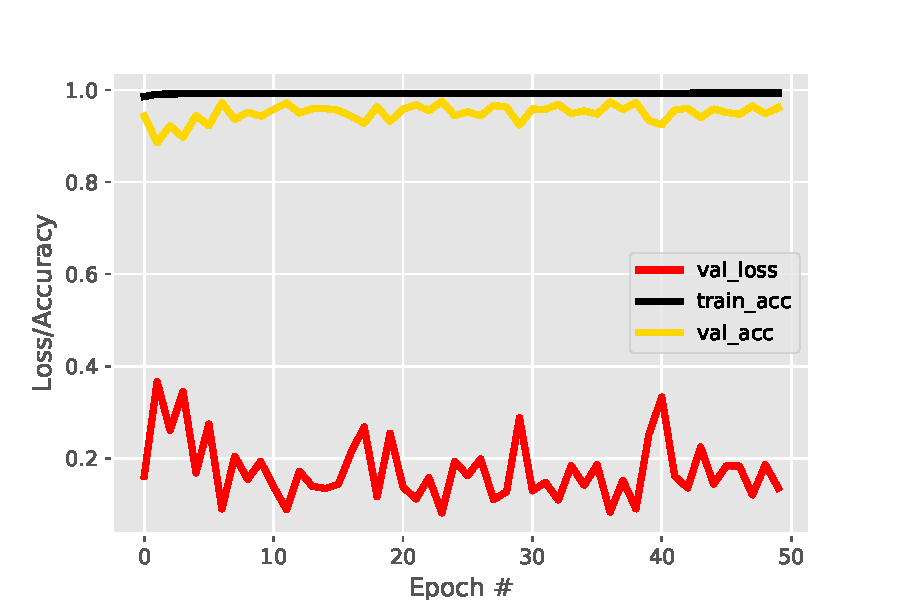
\includegraphics[width=5.8cm]{figs/test_25_val_m1_plot}}{Dataset-0 training}%
\hspace{0.1cm}%
\stackunder[5pt]{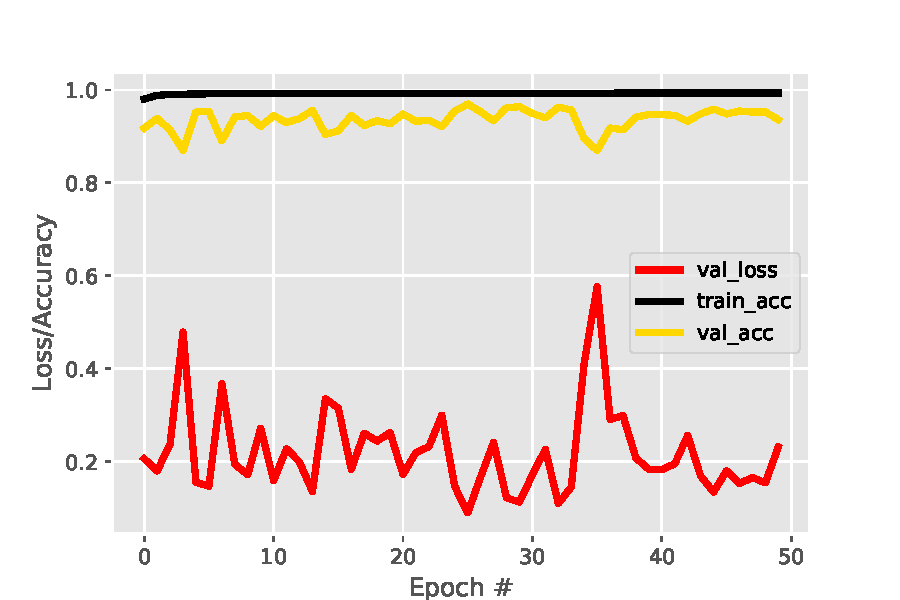
\includegraphics[width=5.8cm]{figs/test_75_val_m1_plot}}{Dataset-1 training}
  
\end{figure}

\scriptsize
 \begin{itemize}
 \item Showing scores during VL mode when classes are split equally for 
validation.
\item Weights selected using lowest VL.
 \item Dataset-0 Validation Samples (7947) for each class.
  \item Dataset-1 Validation Samples (2617) for each class.
 \end{itemize}


\end{frame}
%%%%%%
\begin{frame}
  \frametitle{Results -- Conventional DNN Training}

    \begin{table}
\centering

   \scriptsize Conventional DNN training method precision, recall, and number of test samples
   \\
    \label{tbl:dnn_results}
\begin{tabular}{ |l|l|l|l|l| }
 \hline
Dataset & Class & Precision & Recall & Samples\\ \hline
\multirow{2}{*}{0} 
 & Fire & 0.90 & 0.90  & 26356 \\
 & No-Fire & 0.99 & 0.99 & 427115 \\ 
 \hline

\multirow{2}{*}{1} 
& Fire & 0.00 & 0.00 & 78702 \\
 & No-Fire & 1.00 & 1.00 & 1282862 \\
\hline
\end{tabular}
\end{table}
  \vspace{-0.2cm}
\begin{figure}[ht]
    \scriptsize
\stackunder[5pt]{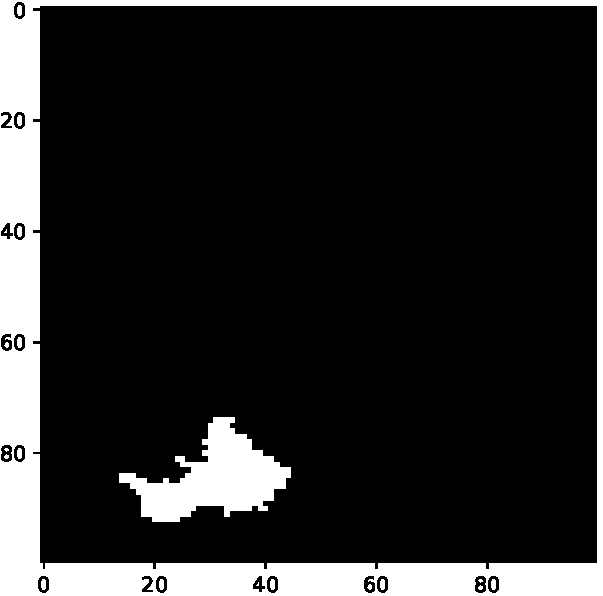
\includegraphics[width=2cm]{figs/test_mask}}{Test Image}
\hspace{0.1cm}%
\stackunder[5pt]{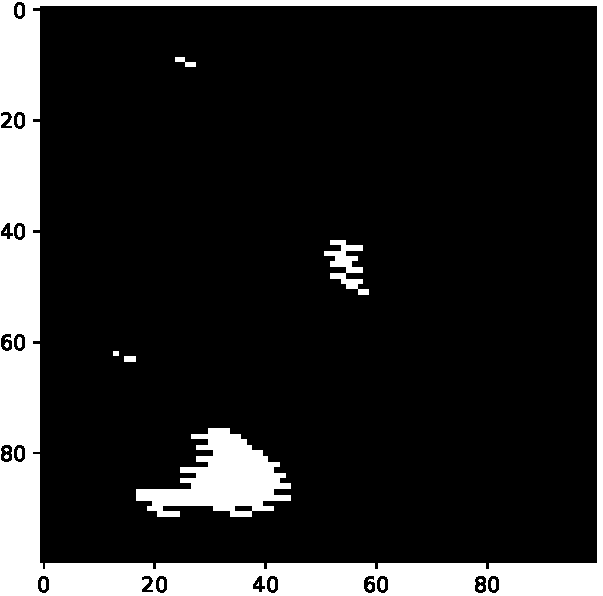
\includegraphics[width=2cm]{figs/test_25_b0m0}}{Dataset - 0}
\hspace{0.1cm}%
\stackunder[5pt]{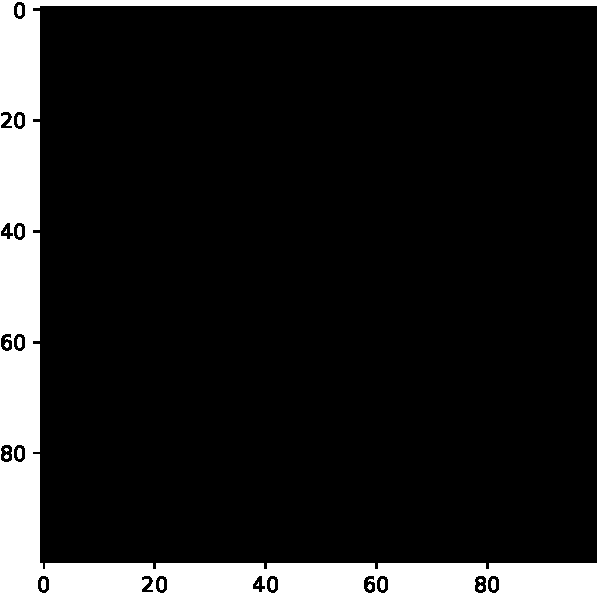
\includegraphics[width=2cm]{figs/test_75_b0m0}}{Dataset-1}

\label{fig:map_dnn_vl}
\end{figure}

\begin{figure}
  \scriptsize
  \stackunder[5pt]{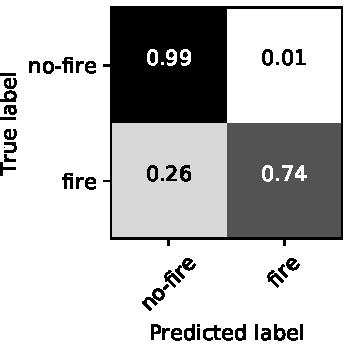
\includegraphics[width=2.5cm]{figs/test_25_b0m0_cm}}{Dataset-0 single fire}
\hspace{0.1cm}%
  \stackunder[5pt]{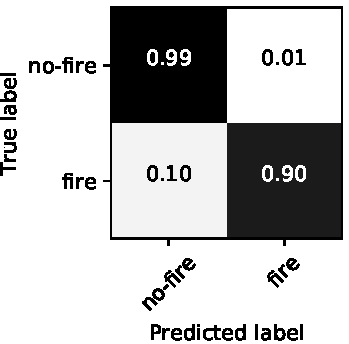
\includegraphics[width=2.5cm]{figs/test_25_b0m0_cm_all}}{Dataset-0 all}
\hspace{0.1cm}%
\stackunder[5pt]{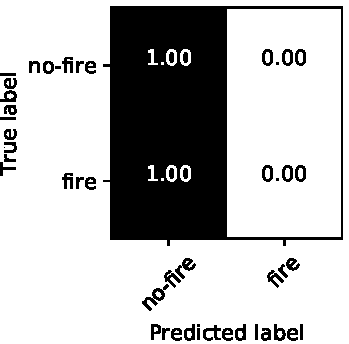
\includegraphics[width=2.5cm]{figs/test_75_b0m0_cm}}{Dataset-1 single fire}
\hspace{0.1cm}%
  \stackunder[5pt]{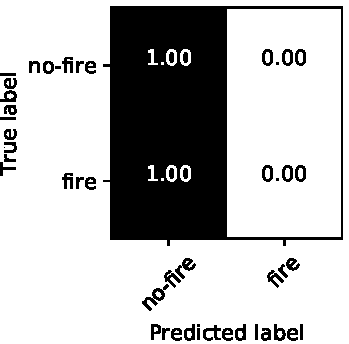
\includegraphics[width=2.5cm]{figs/test_75_b0m0_cm_all}}{Dataset-1 all}
  
\end{figure}
  
\end{frame}

%%%%%%%%%%%%%%%%%%%%%%%%%%%%%%%%%
\begin{frame}
  \frametitle{Results -- VL DNN Training}
  \footnotesize

\begin{table}
\centering

   \scriptsize
VL DNN training method precision, recall, and number of test samples
   \\
    \label{tbl:dnn_results_vl}
\begin{tabular}{ |l|l|l|l|l| }
 \hline
Dataset & Class & Precision & Recall  & Samples \\ \hline
\multirow{2}{*}{0} 
 & Fire & 0.68 & 0.95 & 26356\\
 & No-Fire & 1.00 & 0.97 & 427115\\ 
 \hline

\multirow{2}{*}{1} 
& Fire & 0.61 & 0.96 & 78702\\
 & No-Fire & 1.00 & 0.96 & 1282862\\
\hline
\end{tabular}
\end{table}


  \vspace{-0.2cm}
\begin{figure}[ht]
\scriptsize
\stackunder[5pt]{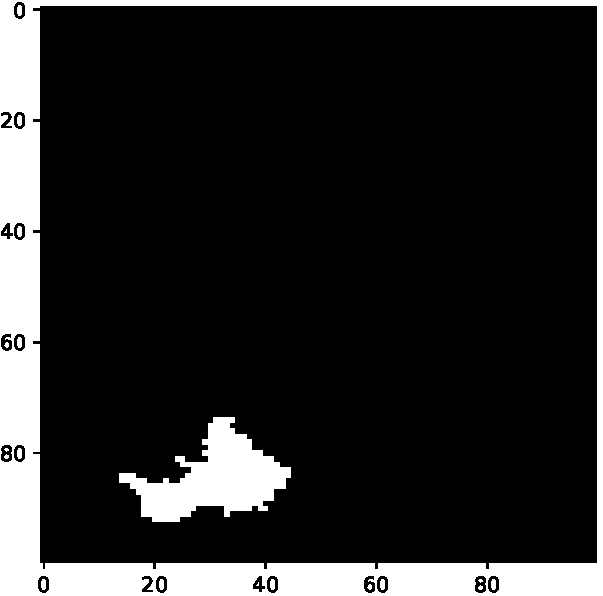
\includegraphics[width=2cm]{figs/test_mask}}{Test Image}
\hspace{0.1cm}%
\stackunder[5pt]{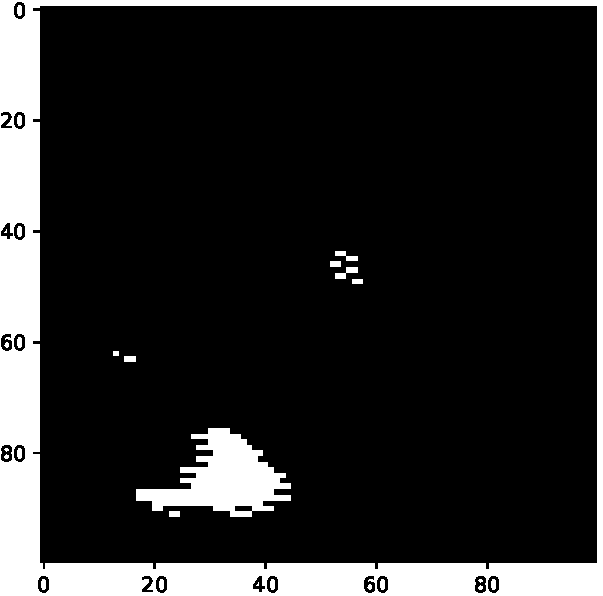
\includegraphics[width=2cm]{figs/test_25_b0m1}}{Dataset - 0}
\hspace{0.1cm}%
\stackunder[5pt]{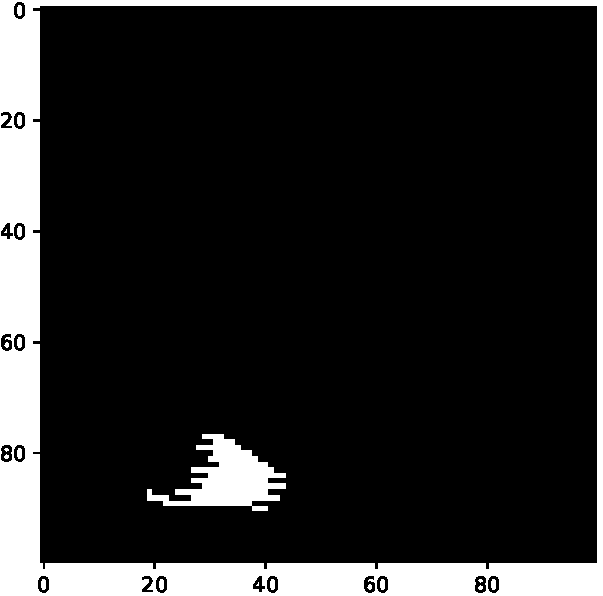
\includegraphics[width=2cm]{figs/test_75_b0m1}}{Dataset-1}

\label{fig:map_dnn_vl}
\end{figure}

\begin{figure}
 \scriptsize
  \stackunder[5pt]{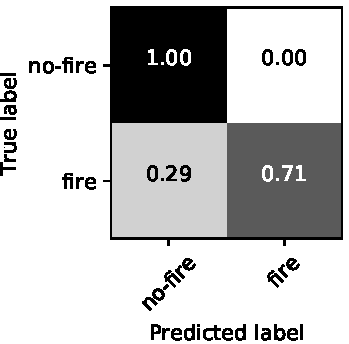
\includegraphics[width=2.5cm]{figs/test_25_b0m1_cm}}{Dataset-0 single fire}
\hspace{0.1cm}%
   \stackunder[5pt]{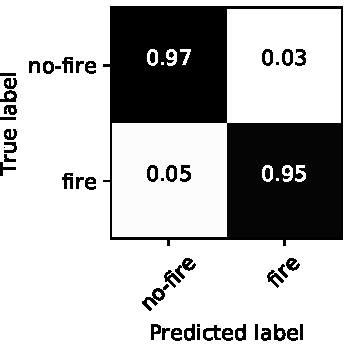
\includegraphics[width=2.5cm]{figs/test_25_b0m1_cm_all}}{Dataset-0 all}
\hspace{0.1cm}%
\stackunder[5pt]{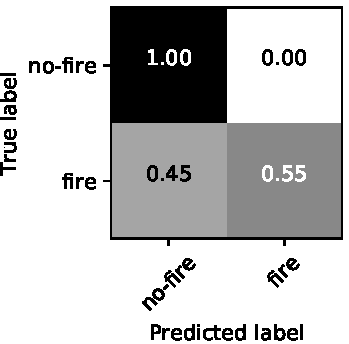
\includegraphics[width=2.5cm]{figs/test_75_b0m1_cm}}{Dataset-1 single fire}
\hspace{0.1cm}%
  \stackunder[5pt]{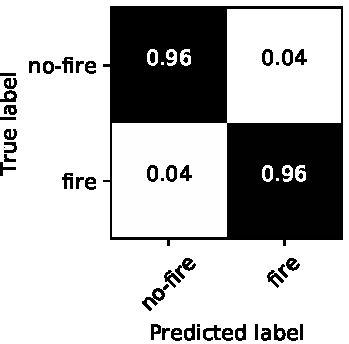
\includegraphics[width=2.5cm]{figs/test_75_b0m1_cm_all}}{Dataset-1 all}
  
\end{figure}
   

\end{frame}


%%%%%%%%%%%%%%%%%%%%%%%%%%%%%%%%%
\begin{frame}
  \frametitle{Results -- U-Net Segmentation}
 \scriptsize
 \begin{itemize}
 \item U-Net is 2D CNN architecture for fast and precise segmentation of images 
\cite{RonnebergerFB15}.
 \item  Consists of a contracting path (left side) and an expansive path (right 
side).
 \end{itemize}

\centering
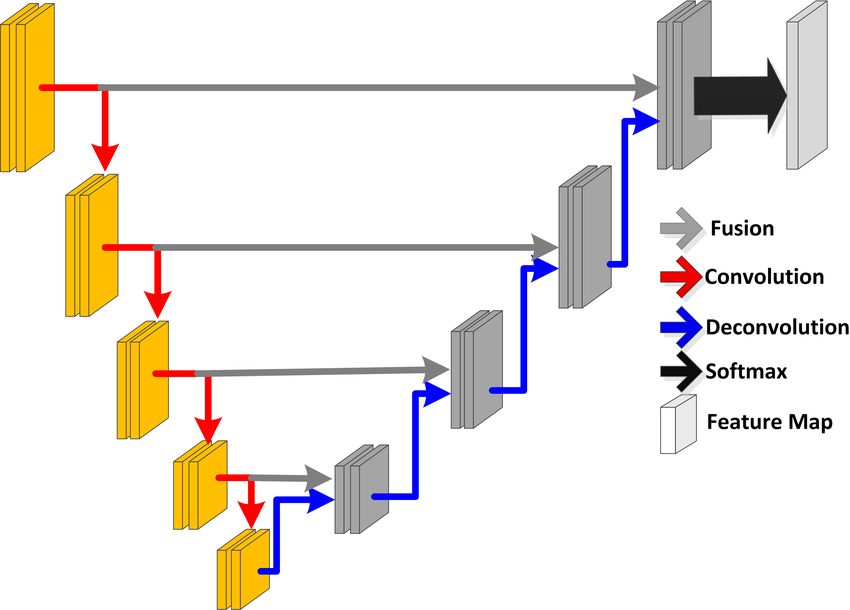
\includegraphics[width=0.5\textwidth]{figs/U-net-architecture.png}


\begin{table}
\centering

   \scriptsize U-Net training method precision, recall, and number of 
test samples
   \\
    \label{tbl:dnn_results}
\begin{tabular}{ |l|l|l|l|l| }
 \hline
Dataset & Class & Precision & Recall & Samples\\ \hline
\multirow{2}{*}{0} 
 & Fire & 0.00 & 0.00  & 518879 \\
 & No-Fire & 0.95 & 1.00 & 27293 \\ 
 \hline

\end{tabular}
\end{table}

\end{frame}  

%%%%%%%%%%%%%%%%%%%%%%%%%%%%%%%%%
\begin{frame}
  \frametitle{Results -- XGBoost Algorithm}
  \scriptsize
   \begin{itemize}
 \item XGBoost is a scalable and accurate implementation of gradient boosting 
machines \citep{Chen:2016}.
 \item  XGBoost used a more regularized model formalization to control 
overfitting.

 \end{itemize}


 
\begin{table}
\centering
   \caption{XGBoost method scores for precision, recall, and number of test 
samples}
    \label{tbl:xgb_results}
\begin{tabular}{c l r r r l}
 \toprule
 \multicolumn{1}{c}{Dataset} & \multicolumn{1}{c}{Class} & 
\multicolumn{1}{c}{Precision} & \multicolumn{1}{c}{Recall} & 
\multicolumn{1}{c}{Samples} & \multicolumn{1}{c}{Region} \\
 \midrule
\multirow{4}{*}{0} 
 & Fire & 0.94 & 0.85  & 26,356 & Study Region\\
 & No-Fire & 0.99 & 1.00 & 427,115 & Study Region\\ 
 
 & Fire & 0.88 & 0.77  & 276 & Single Wildfire\\
 & No-Fire & 0.99 & 1.00 & 9,724 & Single Wildfire\\ 
 \midrule
\multirow{4}{*}{1} 
 & Fire & 0.94 & 0.85 & 78,702 & Study Region\\
 & No-Fire & 0.99 & 1.00 & 1,282,862 & Study Region\\ 
 
 & Fire & 0.88 & 0.76 & 276 & Single Wildfire\\
 & No-Fire & 0.99 & 1.00 & 9,724 & Single Wildfire\\ 
 \bottomrule
\end{tabular}
\end{table}

\centering
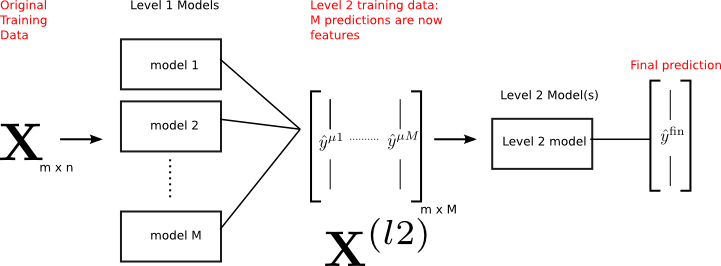
\includegraphics[width=0.4\textwidth]{figs/workflow.png}
\\
\tiny{Source:https://www.kdnuggets.com}


\end{frame}  
%%%%%%%%%%%%%%%%%%%%%%%%%%%%%%%%%
\begin{frame}
  \frametitle{Conclusions and Next Steps}
\scriptsize
	      \begin{itemize}
               \item MODIS bands can be used to predict spatial extents of wildfire with good accuracy.

	       \item Google Earth Engine provides a powerful platform for processing and analyzing datasets without moving data.
	       \item VL DNN training strategy significantly improves performance and possibly captures unknown wildfires outside MTBS dataset. 
	       \item Next steps: more sophisticated algorithms 
utilizing sequential data and meta-learning approaches.  
              \end{itemize}

 
 
     \begin{columns}[T]
    \begin{column}{.5\textwidth}
     
   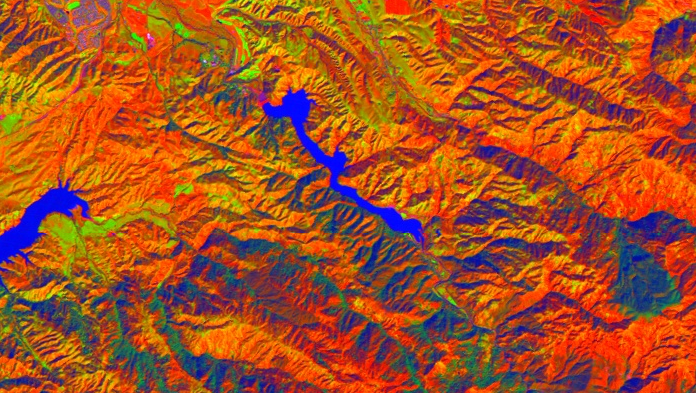
\includegraphics[width=1.0\textwidth]{figs/gee_spectral.png}

   \centering
   \vspace{-0.2cm}

    \end{column}
    \begin{column}{.5\textwidth}
    \vspace{-0.2cm}
    
 
    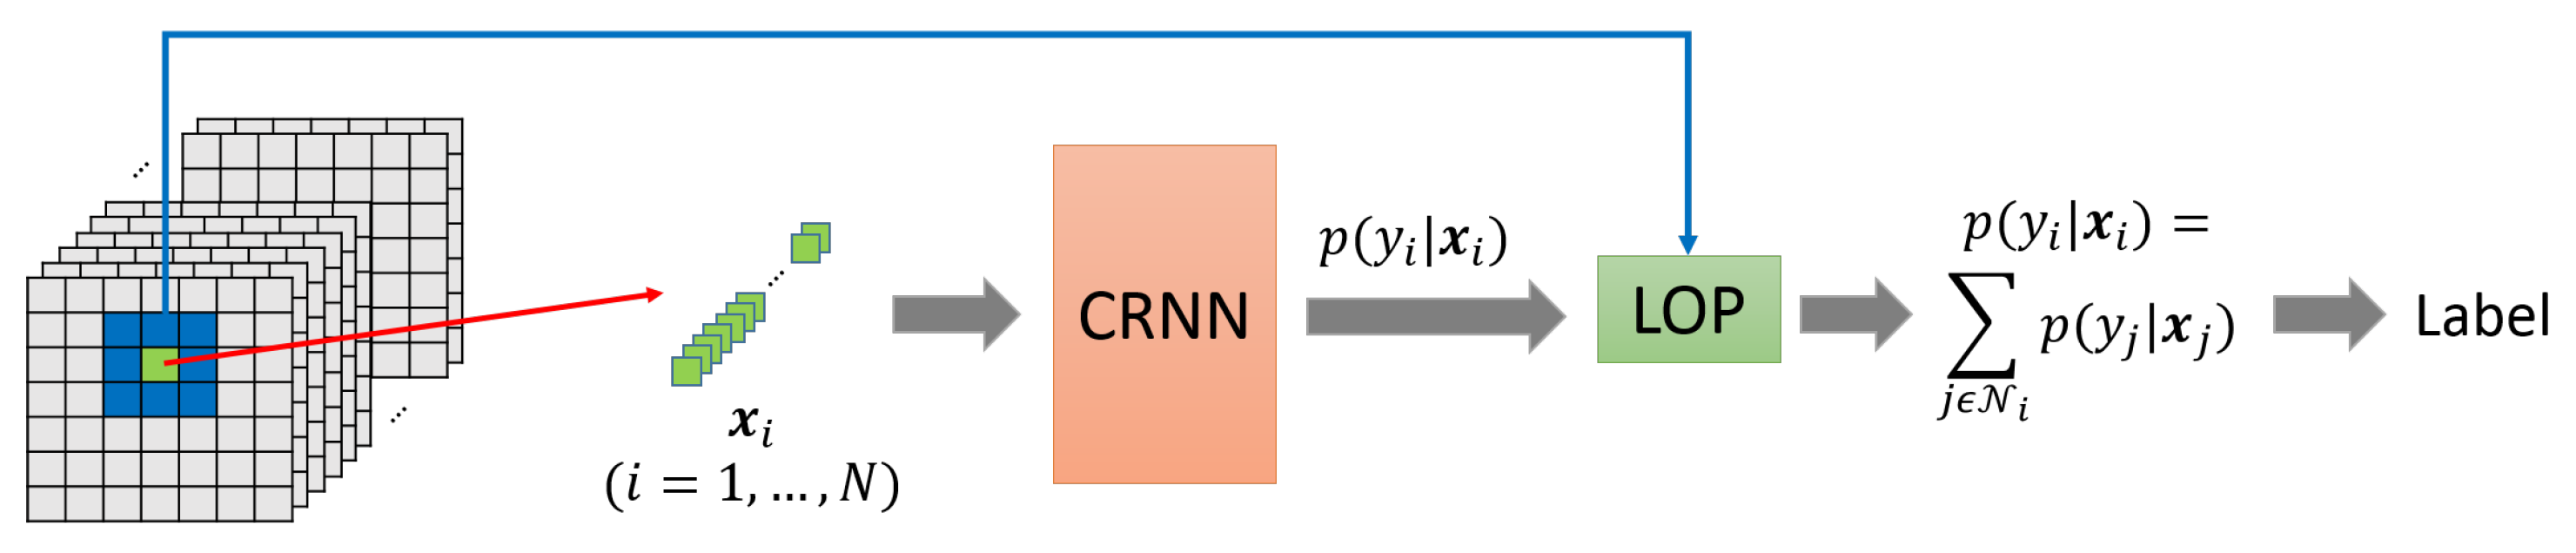
\includegraphics[width=1.0\textwidth]{figs/crnn_rs.png}
\\
\tiny 
\centering
Source: Convolutional Recurrent Neural Networks for
Hyperspectral Data Classification \cite{rs9030298}
   
    \end{column}
  \end{columns}
\end{frame}
%%%%%%%%%%%%%%%%%%%%%%%%%%%%%%%%%%%%%%%%%%%%%%%%%%%%%%%%%%%%%%%%%%%%%%%%%%%%%%%
%\section{Acknowledgments}
%%%%%%%%%%%%%%%%%%%%%%%%%%%%%%%%%%%%%%%%%%%%%%%%%%%%%%%%%%%%%%%%%%%%%%%%%%%%%%%
%%%%%%%%%%%%%%%%%%%%%%%%%%%%%%%%%%%%%%%%%%%%%%%%%%%%%%%%%%%%%%%%%%%%%%%%%%%%%%%
\begin{frame}
 \frametitle{Acknowledgments}\footnotesize
 \begin{center}
  \vskip-0.25in
  
\includegraphics[height=0.70in]{logos/DOE_Office_of_Science_logo.pdf}
%  \hspace{0.25in}
%  \includegraphics[height=0.70in]{logos/USFS_Logo.png}
%  \hspace{0.25in}
%  \includegraphics[height=0.70in]{logos/NSF_logo.jpg}
 \end{center}
 %\vskip-0.10in
This research was supported by
the Next-Generation Ecosystem Experiments (NGEE Arctic)
and
the Reducing Uncertainties in Biogeochemical Interactions through Synthesis and Computation (RUBISCO) Scientific Focus Area (SFA),
which are sponsored by the Climate and Environmental Sciences Division (CESD)
of the Biological and Environmental Research (BER) Program
in the US Department of Energy Office of Science.
Oak Ridge National Laboratory (ORNL) is managed by UT-Battelle, LLC,
for the US Department of Energy under Contract No.\ DE-AC05-00OR22725.

\medskip
\textbf{Code and slides will be available at}
\url{https://github.com/langfordzl/zlangford_icdm2018}

\end{frame}
%%%%%%%%%%%%%%%%%%%%%%%%%%%%%%%%%%%%%%%%%%%%%%%%%%%%%%%%%%%%%%%%%%%%%%%%%%%%%%%


%%%%%%%%%%%%%%%%%%%%%%%%%%%%%%%%%%%%%%%%%%%%%%%%%%%%%%%%%%%%%%%%%%%%%%%%%%%%%%%

%%%%%%%%%%%%%%%%%%%%%%%%%%%%%%%%%%%%%%%%%%%%%%%%%%%%%%%%%%%%%%%%%%%%%%%%%%%%%%%
% References
%%%%%%%%%%%%%%%%%%%%%%%%%%%%%%%%%%%%%%%%%%%%%%%%%%%%%%%%%%%%%%%%%%%%%%%%%%%%%%%
%%%%%%%%%%%%%%%%%%%%%%%%%%%%%%%%%%%%%%%%%%%%%%%%%%%%%%%%%%%%%%%%%%%%%%%%%%%%%%%
\begin{frame}
 \frametitle{References}
 \def\newblock{}
 \renewcommand\refname{}
 %\vbox{\Large References}
 \vskip-0.12in
 {\scriptsize
  \bibliographystyle{abbrvnat}
  \bibliography{refs/abbrev,refs/link_doi,refs/references}
 }
\end{frame}
%%%%%%%%%%%%%%%%%%%%%%%%%%%%%%%%%%%%%%%%%%%%%%%%%%%%%%%%%%%%%%%%%%%%%%%%%%%%%%%

%%%%%%%%%%%%%%%%%%%%%%%%%%%%%%%%%%%%%%%%%%%%%%%%%%%%%%%%%%%%%%%%%%%%%%%%%%%%%%%

\end{document}
